%
% Documento: Introdução
%

\chapter{Introdução}\label{chap:introducao}  

Define-se mobilidade como aquilo que tem “facilidade de se movimentar, andar, dançar.” \cite{mobilidade}, característica do que é móvel ou obedece às leis do movimento. Mobilidade Urbana já é um termo que não encontramos no dicionário, porém de fácil compreensão quando analisamos as duas palavras juntas, pois logo relacionamos
a algo que de fato é ou se assemelha, basicamente a condição 
de se deslocar dentro de uma cidade, campus, bairro. %com objetivo de criarmos relações sociais, — como ir ao supermercado —, ou relações econômicas — como ir ao trabalho —, utilizando meios de transporte como carros, ônibus, metrô, etc.



No Brasil, com a Política Nacional de Mobilidade Urbana - PNMU, % \footnote{Disponível em: url{http://www.planalto.gov.br/civil_03/_ato2011-2014/2012/lei/l12587.html}. Acesso em: 07 de Jun. 2021}
aprovada em 2012, obriga estados e municípios com mais de 20 mil habitantes a terem um planejamento de expansão pensando em como as pessoas vão se locomover, considerando o crescimento urbano e populacional  \cite{lei12587}. %Assim, cabe ao poder público elaborar este projeto considerando todos os direitos dos cidadãos.

\begin{comment}
Alguns desses direitos é tornar as vias uma forma de liberdade aos cidadãos, garantir o direito de ir e vir, adaptar ruas, adaptar ciclovias, adaptar calçadas, adicionar novos meios de transporte, e etc. %A exemplo disso, podemos citar o Uber \footnote{Disponível em: https://www.uber.com/br/pt-br/. Acesso em: 23 Jun. 2020}, que é um aplicativo de transporte que entra como uma solução de mobilidade urbana.
	conteúdo...
\end{comment}

Segundo informe do Instituto de Pesquisa Econômica Aplicada - IPEA, o aumento da produção automotiva no Brasil estimulou a crescente utilização de carros e motos em todo o território nacional. O fácil acesso a esses automóveis provocou a redução da importância do transporte público na matriz modal, aumentou o tráfego e a emissão de poluentes \cite{ipea}.

%É neste cenário 
%de problemas 
%urbano que surge 
As Cidades Inteligentes - CIs, hoje são vistas como uma das soluções para alguns problemas urbanos. %,tendo Mobilidade Inteligente como um dos seus aspectos. 
As CIs buscam sempre melhorar o estilo de vida dos cidadãos, ao administrar recursos, analisar a qualidade do ar, gerenciar resíduos, controlar o trânsito, entre outros \cite{chourabi}.
%Estes e infraestruturas inadequadas  
%estão entre as medidas mais assistidas por Cidades Inteligentes \cite{chourabi}.

De acordo com \citeonline{namepardo}, o conceito de CIs não chega a ser uma novidade no mundo acadêmico e já é amplamente discutido, mas  ganhou uma nova dimensão a partir do momento que passou a implementar Tecnologias da Informação e Comunicação - TICs para construir e integrar infraestruturas e serviços de uma cidade.	
%, surgindo assim iniciativas de CIs como modelos para mitigar e remediar os atuais problemas urbanos. 
%e fazer cidades melhores como lugar para viver.

Tecnologias como GPS e \textit{Smartphones} são tendências no atual momento das cidades inteligentes, estes dispositivos propiciam a criação de novas soluções inteligentes. Com o recurso do GPS, a capacidade de localizar ou buscar endereços nos mapas digitais facilitam bastante ao planejar um trajeto, recurso este que é utilizado por serviços como Google Maps\footnote{Disponível em: https://www.google.com.br/maps. Acesso em: 20 Jun. 2020.}.

Então, com o fim de amenizar o impacto dos combustíveis fósseis e facilitar o trajeto das pessoas, a mobilidade urbana se uniu à Mobilidade inteligente que é um dos conceitos de CIs que utiliza recursos tecnológicos para resolver problemas relacionados a Mobilidade.

Esse conceito envolve acessibilidade, soluções modernas e sustentabilidade, com forte suporte tecnológico para facilitar os deslocamentos, especialmente em grandes centros urbanos.

%que disponibiliza inúmeros pontos comerciais e suas rotas de acesso de acordo com a localização atual do usuário, aplicativos de compartilhamento de veículos (MoObie\footnote{Disponível em: https://moobie.com.br %/?campaignid=11670172030&adgroupid=112146735343&adid=483900492395&gclid=Cj0KCQiAvvKBBhCXARIsACTePW9MWhsrLutbfyQZXSOWv95-wUh_6RE_ClIkiJjaQ8buRpbOFbNHd-gaAjukEALw_wcB. 
%. Acesso em: 25 Nov. 2020}), aplicativos que oferecem trajetos, localização de coletivos e previsão de deslocamento (Cittamobi\footnote{Disponível em: https://www.cittamobi.com.br/home/. Acesso em: 23 Jun. 2020.}, Moovit\footnote{Disponível em: https://moovitapp.com/belem-3183/poi/pt-br. Acesso em: 23 de Jun. 2020.}).

\begin{comment}
Então, com o fim de amenizar o impacto dos combustíveis fósseis e facilitar o trajeto das pessoas, a mobilidade urbana se uniu à Mobilidade inteligente que é um dos conceitos de CIs que utiliza recursos tecnológicos para resolver problemas relacionados a Mobilidade. Já existem algumas soluções. 
%voltadas para o uso de tecnologias sustentáveis,
%uma delas é utilizando aplicações de navegação multimodal possibilitando a escolha da melhor rota \cite{silva2019}%
Soluções como programas de incentivo ao compartilhamento de bicicletas \cite{itau2013}\footnote{Disponivel em: https://www.itau.com.br/imprensa/releases/pe-implanta-1-programa-de-compartilhar-bicicletas-intermunicipal-do-pais.html. Acesso em: 23 Jun. 2020.}, patinetes elétricos \cite{santospereira}, carros elétricos \cite{kon}, por meio de ferramentas de planejamento de viagens com o transporte público como o Cittamobi\footnote{Disponível em: https://www.cittamobi.com.br/home/. Acesso em: 25 nov. 2020}, são algumas destas soluções. 
%compartilhamento de carros elétricos como VAMO (Veículos Alternativos para Mobilidade) Fortaleza \footnote{Disponível em: http://www.vamofortaleza.com/. Acesso em 25 Nov. 2020}, soluções de iniciativas privadas como o Uber e 99\footnote{Disponível em: https://99app.com/. Acesso em: 01 Mar. 2021},
% aplicativos que oferecem a mobilidade como um serviço
%e que utilizam tecnologias que calculam a melhor trajeto
%— a exemplo do Uber e 99 — 
%aplicativos de carona como o BlaBlaCar\footnote{Disponível em: https://www.blablacar.com.br/. Acesso em: 28 Nov. 2020} que oferece viagens de longa distância, entre outros \cite{carpooling2013}.
%que utilizam da proximidade entre o motorista e o passageiro — compartilhar o carro com um colega de trabalho ou vizinho que mora perto — sem cobrar nada ou apenas um valor simbólico.
\end{comment}

% -------------------------------------
\begin{comment}
A proposta de uma cidade inteligente nada mais é do que aprimorar recursos e serviços de uma região utilizando TICs, tornando mecanismos que envolvem a gestão de recursos e serviços mais eficiente, sustentável e melhorando a qualidade de vida \cite{kon}. Decorrente do crescimento da população nas cidades, surgiram problemas nas áreas urbanas oriundos desse crescimento, com a necessidade de encontrar alternativas para tentar sanar os problemas, as cidades inteligentes, e especialmente a mobilidade inteligente tiveram destaques, junto a isso \cite{silva2019}, o conceito de mobilidade como serviço \cite{jittrapirom} e compartilhamento de caronas e corridas (Consumo Colaborativo) aparecem como alternativas.
\end{comment}
% -------------------------------

%Neste trabalho, será focado o aspecto da Mobilidade Inteligente, no Capítulo 2 será explicado como será desenvolvido o projeto, as etapas concluídas e o que está pendente. No capítulo 3 discutiremos os conceitos que aproximam o trabalho, falaremos um pouco mais de cidade inteligente, mobilidade inteligente, e ainda será comentado sobre Campus Inteligente.
% 
%\mnote{Patrícia: evita falar na primeira pessoa do singular. Usa a primeira pessoa do plural ou orações passivas do tipo "será discutido tal coisa...".}
    %

%O capítulo 4 é sobre os trabalhos relacionados a este projeto. O Capítulo 5 trata da proposta do projeto, dos dados obtidos, das características da proposta, das dificuldades enfrentadas até aqui e dos próximos passos e para finalizar no capítulo 6 contêm o cronograma de execução.

\section {Problema}
\begin{comment}
	Na cidade de Macapá e Santana, as duas maiores cidade do Amapá, o número de transporte coletivo é baixo,
	existe apenas duas rodovias que interligam as cidades, 
	se locomover se torna difícil \cite{sau2018}. % 
	
	Com tantos problemas aparentes causadas pelo grande inchaço populacional que  vive nas áreas urbanas, cerca de 80\% da população das duas cidades reside em áreas urbanas e sofre com a insuficiência do sistema de transporte público oferecido \cite{tostes}.
\end{comment}




Macapá, a cidade onde se encontra o campus,  entre os  anos de 2010-2017 teve um crescimento total de 13 ônibus ativos, e nesse mesmo período houve um aumento de 57.967 pessoas somente na cidade de Macapá. 

Esses alunos tem como transporte público os ônibus e taxis, e no caso de Santana, a cidade vizinha, os alunos tem apenas uma linha de ônibus que faz a rota intermunicipal. \cite{sau2018}.


%e cerca de 80\% da população reside em Macapá e Santana, cidade vizinha que muitos alunos estudam na Unifap e tem como transporte público legalizado apenas o ônibus e táxis. 
%sendo que a Companhia de Transporte de Macapá (CTMAC) apontou nesse mesmo período um crescimento de 57.967 pessoas\cite{sau2018}.
 
Em Macapá, muitas rotas não assistem todas as áreas da cidade, sendo necessário necessário replanejar seu itinerário, pegar outro ônibus ou meio de transporte, aumentando ainda mais o tempo de uso do transporte coletivo para chegar ou sair da Unifap. \cite{galiano}.

Na pesquisa que realizada, na pergunta "Quais os principais problemas enfrentados com o transporte que utiliza?", o principal problema apontado pelos entrevistados foi o tempo gasto, que somou 80\% de todas as pessoas que responderam a pergunta.

%Pensando nesse problema que optamos por um estudo de mobilidade inteligente, buscando as alternativas atuais que ajudam aos acadêmicos da Unifap a chegarem o saírem da universidade. 
% a diminuir os atuais problemas encontrados com a mobilidade, só que este, resolvendo problemas da Unifap, com um ambiente menor, o ambiente de um Campus Inteligente.

%\mnote{Patrícia: falta concluir aqui com algo como: "com isso, o estudo de soluções de mobilidade inteligente pode trazer... blablabla" e então relacionar o problema com a Unifap.}


\begin{comment}
Adicionar contexto da unifap e Macapá - incluir a quantidade de pesosas que pegam onibus diariamente e a quantidade de alunos que pegam na unifap
\end{comment}



\section{Justificativa}

%A qualidade do transporte público no Brasil não é das melhores, existe muita demora no transporte,  ônibus precários, tarifas altas, superlotação em toda parte do país, e no Amapá, o cenário é bem similar ao de grande parte do país%
	%\mnote{Patrícia: não coloca nenhum texto que tenha uma expressão a opinião pessoal. Eu apagaria todo esse texto inicial e começariam com o texto abaixo.}
    %
 Segundo \citeonline{tostes} a grande concentração populacional em áreas urbanas, cerca de 90\% e especialmente em Macapá agrava problemas sociais e deixa mais claro e evidente a deficiência do transporte público local. Isso atinge em cheio a qualidade de vida da população e o meio ambiente~\cite{sau2018}.

Sabendo que a cidade de Macapá possui um baixo número de coletivos, um grande fluxo de veículos principalmente na área central onde o espaço para trafegar é mínimo, problemas como superlotação de ônibus e atrasos são comuns. \citeonline{sau2018} afirma que Macapá não possui outras opções de transporte coletivo, apenas lotações (corridas ilegais), mototaxistas, taxistas e agora aplicativos de compartilhamentos de carro, porém, estes em um custo mais alto.

Considerando que os problemas de mobilidade existentes atualmente em Macapá atingem diretamente a comunidade acadêmica da Universidade Federal do Amapá, este trabalho buscará entender o perfil e as principais dificuldades da comunidade acadêmica, e, a partir de um estudo de soluções existentes no contexto de CI, propor uma solução que seja viável e admissível para a comunidade acadêmica da Unifap

%E para somar
%Além disso, os altos índices de criminalidade 
%afligem a população que precisa do transporte coletivo, principalmente à noite em paradas escuras
%, realidade da parada que se localiza em frente à Universidade. Muitos alunos sofrem da falta de ônibus ou de apenas uma empresa cobrir a área onde o estudante mora, e ainda existe na cidade muitas áreas sem uma empresa de ônibus cobrindo a área.  [foto ou materia que fale dessa situação]
%	\mnote{Patrícia: infelizmente não temos como afirmar isso sem uma referência e dados concretos. Melhor retirar esse parágrafo.}
    %

\begin{comment}
\textit{\textbf{NOTA - Poderia finalizar com um texto mais ou menos assim:}
Considerando que os problemas de mobilidade existentes atualmente em Macapá atingem diretamente a comunidade acadêmica da Universidade Federal do Amapá, este trabalho buscará entender o perfil e as principais dificuldades da comunidade acadêmica, e, a partir de um estudo de soluções existentes no contexto de cidades inteligentes, propor uma solução que seja viável e admisível para a comunidade acadêmica da Unifap....
\textbf{Algo assim.}}

\end{comment}

\begin{comment}
Com a intenção de apresentar uma alternativa de mobilidade à comunidade acadêmica da Universidade, a proposta de aplicativo de caronas tem como objetivo dar mais uma opção de transporte de entrada e saída dos alunos, professores e técnicos da Unifap.
\end{comment}
%Para isto, foi realizada uma pesquisa através de um formulário utilizando a ferramente \textit{Google Forms}. Este formuçário foi criado para coletar a opinião dos alunos, professores e técnicos da universidade a respeito da proposta de um aplicativo e carona solidária para a universidade, e obtivemos várias em relação aos motivos para aderir à iniciativa dentro do campus Macapá.%



\section {Objetivos}

\subsection{Objetivo Geral}

Este trabalho tem como objetivo principal o estudo sobre Mobilidade Inteligente
%, de viabilidade 
%considerando o que se entende sobre Cidades Inteligentes, 
considerando o contexto de mobilidade relacionado à Universidade Federal do Amapá
%para a proposta do aplicativo de carona solidária para a Unifap, 
e realizar o debate sobre a viabilidade de utilização pela comunidade acadêmica em geral (docentes, discentes e técnicos) de soluções tecnológicas existentes, visando oferecer alternativa(s) de transporte que dê acesso e diminua problemas diários enfrentados para chegar e/ou sair da universidade.
%com outros modais utilizados (ônibus, bicicleta, moto, etc.).

\subsection{Objetivos Específicos}

Para alcançar o objetivo geral, definimos os seguintes objetivos específicos:

\begin{enumerate}
\item Estudo sobre Cidades Inteligente focado em Mobilidade Inteligente;
\item Realizar um levantamento de soluções de Mobilidade Inteligente;
\item Levantamento sobre o perfil da comunidade acadêmica da Unifap;
\item Análise comparativa dos diferentes tipos de soluções de Mobilidade Inteligente considerando o perfil da comunidade acadêmica da Unifap;
\item Definir os requisitos da solução mais viável para a comunidade acadêmica da Unifap;
\item Definir a proposta de projeto de solução de Mobilidade Inteligente considerando o perfil da comunidade acadêmica da Unifap;
\item Levantamento das soluções disponíveis que se encaixam dentro dos requisitos;
\item Triagem das soluções encontradas;
\item Teste da solução escolhida;

\end{enumerate}

\begin{comment}


\begin{enumerate}
\item \textit{Realizar um questionário.}
\item \textit{Analisar os resultados do questionário.}
\item \textit{Preparar o ambiente de desenvolvimento.}
\item \textit{Estudar as ferramentas que serão utilizadas no projeto.}
\item \textit{Procurar soluções similares com o objetivo de tirar ideias utéis para o projeto.}
\item \textit{Verificar soluções que já existem com a mesma proposta de caronas solidárias, reutilizar código se for de código aberto.}
\item \textit{Integrar os serviços de gestão acadêmica com a ferramenta que irá ser criada/reutilizada na proposta.}


\end{enumerate}
\end{comment}




%Na Figura \ref{bigdata}, temos:

%\begin{figure}[!hbtp]
%	\centering
%	\caption{Perspectivas de \textit{big data}.}
%	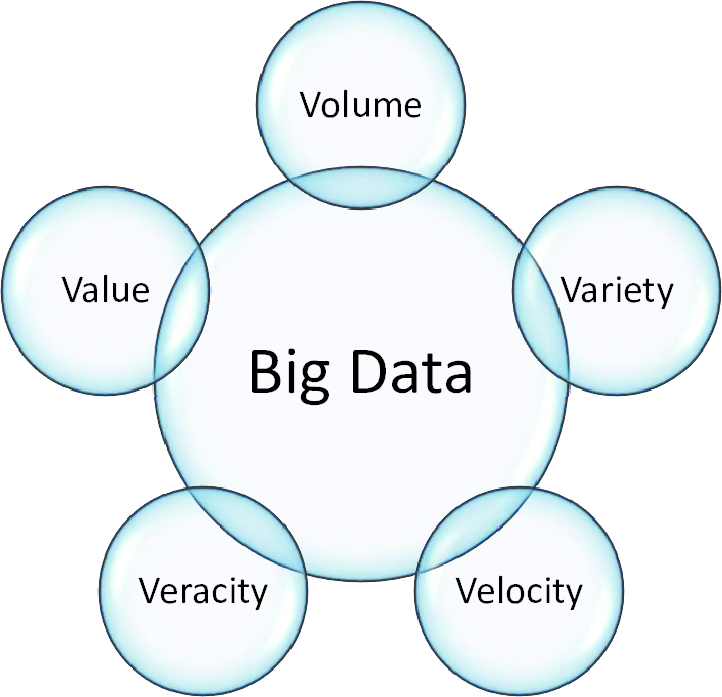
\includegraphics[scale=.75]{./04-figuras/bigdata.png}
%	\label{bigdata}
%	\fonte{\cite{elragal:2014}}
%\end{figure}



%\section {Exemplo de Seção}

%\subsection{Exemplo de Subseção}

%\subsubsection{Exemplo de Subseção da Subseção}

%\section {Tabela}
%Na Tabela \ref{tabela}, temos: 

%\begin{table*}[ht]
%	\centering
%	\caption{Exemplo de Tabela.}
%	\label{tabela}
%	\begin{tabular}    %{p{0.49\linewidth}p{0.03\linewidth}p{0.03\linewidth}p{0.03\%linewidth}p{0.03\linewidth}p{0.21\linewidth}}
%		\hline
%		Ítem & Ítem & Ítem & Ítem & Ítem & Ítem\\
%		\hline
%		Ítem & Ítem & Ítem & Ítem & Ítem & Ítem\\
%		\hline
%	\end{tabular}
%\end{table*}